\chapter{The Basics}
	In general the \de{design} is a synthesis of a new concept (or as arrangement of existing solutions) in order to realise a product which satisfies a recognised need. The design process analysis and defines solution to problems not previously solved or propose new solutions to already solved problems. In particular a \de{mechanical design} is the conceptual resolution of all the problems associated to the construction, testing and commission of a machine.
	
	A \de{machine} can be defined as a system of mechanisms and components that works together in order to accomplish a specific objective; a machine can be subdivided in \textbf{machine elements} that are more or less complex components capable of performing one or more functions (as example a joint system, a revolute pair, a power transmission...).

	\vspace{3mm}
	The \de{engineering design} is the process of devising a system, component or process to meet desired needs; this decision-making process is often iterative, in which the engineering sciences and mathematics are applied to convert resources optimally to meet a stated objective. Any good \textit{design process} should allow even the most complex design to be broken up into manageable stages that encourage and catalyse free-spirited creative thinking and \textbf{deterministic analysis}. A deterministic design, facilitated through the use of a structured design process, is adopted to minimize uncertainty, and hence risk
	

\section{Phases of the design process}
	The design process is iterative in a way that for each step we have new specific information that has to be design processed and, if evaluated badly it might be better to change the solution (or even going backword in the design steps) but if correct it's maybe good to go to the other step. In general, in a design process, the following 10 steps should be considered:
	\begin{enumerate}
		\item \textbf{recognize the need}: this is the general statement made by the client that allow to create the goal of the design;
		
		\item  \textbf{problem definition}: at this point it'n necessary to define the problem specification, and in particular: the objective and goals, the constraints and the criteria used to evaluate the design.\\
		At this stage there are a lot of consideration that might be considered, like strength, costs, reliability, thermal properties... At this stage we have to elaborate the \de{product design specification} \textbf{PDS} containing the requirements that must be met to make the product; this file contains the requirements of the client (derived from the needs and/or the priorities), the design characteristic, the aims/pergormances and the constraints/shortcomings that has to be avoided. In particular this document, that's usually regulated by various norms, must contain:
		\begin{multicols}{2}
			\begin{itemize}
				\item the ID reference, the date and the responsible;
				\item a summary;
				\item a list of content and/or symbols;
				\item an introduction stating the general criteria that guided the compilation of the PDS (motivated by the objective of the product development);
				\item the performances (in a quantitative or qualitative manner) of the machine and it's minimum/permitted/normal operating values;
				\item the constraints of the problem;
				\item transport and mounting condition
				\item the test mode;
				\item the employment training, inspection interval, the maintenance and spare parts;
				\item insurances and timing;
				\item attachments.
			\end{itemize}
		\end{multicols}
	
		\item \textbf{gather information}: this is a never-ending process for the best design engineers that's done through textbooks, journal and magazines, technical reports, company catalogues, web pages, people... and allow the engineer to learn new design methods/techniques and other general informations;
		
		\item \textbf{concept generation}: this is the start of the conceptual study of the machine in order to achieve a solution; in this creative part it's a good idea to sketch design ideas in a logbook. Some \textbf{approaches} to concept generation are
		\begin{multicols}{2}
		\begin{itemize}
			\item \textbf{adaptation} of an already existing solution that works in another field;
			\item \textbf{area thinking} by improving  existing products by concentrating on one of it's important characteristics (like cost, performance, function...);
			\item \textbf{brainstorming};
			\item \textbf{involvement} and it's made by visualizing yourself as being part of the mechanism.
			\item \textbf{inversion} by trying to reverse the ordering of things (\textit{the last become the first});
			\item \textbf{functional synthesis} by dividing the system in subunits that are described independently with their functional requirements and a relative solution.
		\end{itemize}	
		\end{multicols}
		At this stage a useful tool is the \de{FRDPARRC} (\textit{Fred Park}) \de{table}, so one dedicate sheet to each function and it contains 
		\begin{multicols}{2}
		\begin{itemize}
			\item the functional requirements;
			\item the design parameters;
			\item the analysis;
			\item references;
			\item risks;
			\item counter-measures.
		\end{itemize}
		\end{multicols}
		Based on this table we can choose the \textit{correct} strategy to solve the problem by determining the strategy and the concept.
		
		\item \textbf{concept selection}: this stage can be guided with the \de{decision matrix} that unbiasedly evaluated different ideas based on weighted set of objectives the design team decides are important for solving the problem.
		\begin{figure}[bt]
			\centering 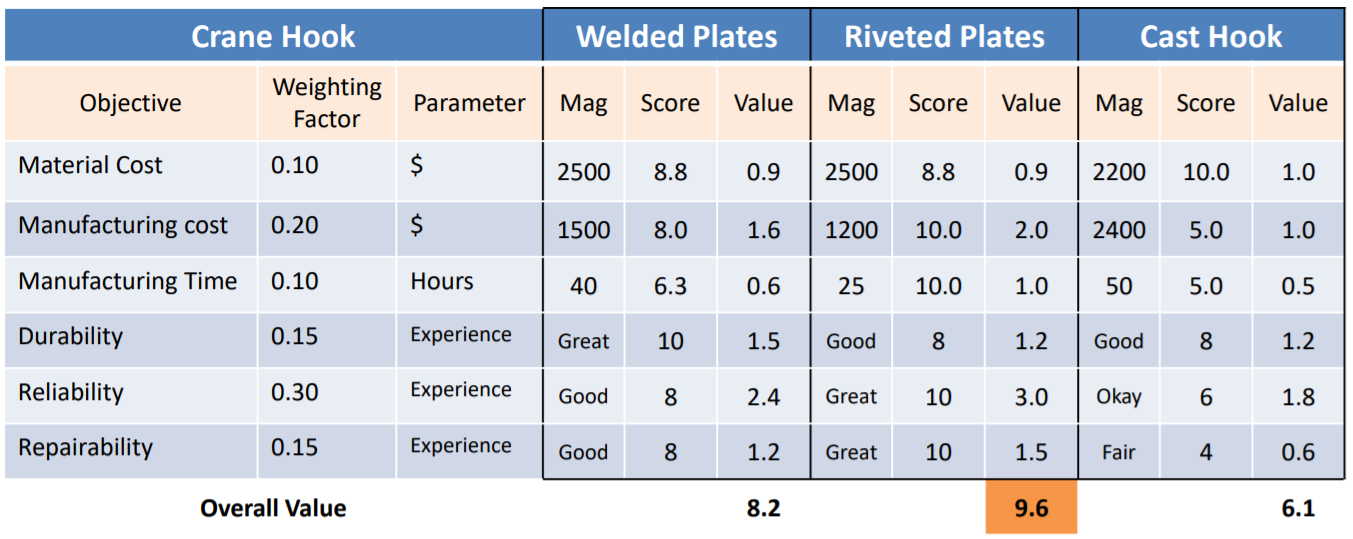
\includegraphics[width=10cm]{decisionmatrix}
			\caption{example of a decision matrix.} \label{fig:bas:decisionmatrix}
		\end{figure}
		As in figure \ref{fig:bas:decisionmatrix}, to create a decision matrix it's necessary to determine a list of objectives with their relative weighting factor (that must sum up to $100\%$). In case of qualitative score assignments it's useful to create another table that match the adjective with a score (for example great $=10$, good $=8$...);
		
		\item \textbf{communication}: the purpouse of this stage is to communicate the decision to the client in order to discuss if the design satisfies it's needs. Designer must provide oral presentations and written design reports. There are only 3 forms of communication that have to be mastered: written, oral and graphical (in particular the ability of creating sketches, drawings... is the best to transmit a message);
		
		\item \textbf{detailed design and analysis} of the particular chosen machine: once that the project is defined it's time to develop in practise the machine. In this steps it's important also the mathematical/physical representation of the system (and no much approximation should be done). At this stage it's important do define all the choices related to  arrangements, shapes, dimensions, tolerances, surfaces finished... but also on load/mechanism analyses (including sizing and verification), planning (time and costs) and relationship among corporate functions.
		
		\item \textbf{prototype and testing}: this is the start of the so calleed \textbf{embodiment phase}. The testing is required to attest the achieved performance, reveal defects, acquire information for an estimate of the service-life and maintenance cycles. This consist of test prior and/or after the installation.
		
		\item \textbf{manufacturing};
		\item \textbf{life cycle maintenance}.
		
	\end{enumerate}
	
	The design activity must provide the final product with technical requirements of performance, but also as \textbf{safety} and \textbf{health} of workers and consumers. In this way the European Commission has defined a harmonised \textbf{regulatory framework} for the design and construction of machine which the designer and manufacturer must refer to: the \texttt{Machine Directive 2006/42/CE}.\\
	The designer must also take into account existing \textbf{standard} (used to achieve uniformity, efficiency and quality of parts/materials/processes) and \textbf{codes} (specification for analysis, design, manufacture and construction to ensure a certain level of safety, efficiency, performance, quality).
	
\section{Design documentation}
	The \de{design documentation} consists in a different set of reports and documents:
	\begin{itemize}
		\item the working \textbf{drawings} of the components;
		\item the \textbf{assembly} drawings;
		\item the \textbf{technical report};
		\item the \textbf{BOM} (Bill of Material) and assembly list;
		\item the use and maintenance handbook.
	\end{itemize}

	In particular the technical report is the document that describes all the choices, the calculations done, the prescriptions and contains the drawings in the annex. The drawings provide the working representation of the components and their assembly drawings (group or total) with the relative assembly lists and description of assembly cycles.
	
	This technical report must contain all of the following point:
	\begin{enumerate}
		\item the title, the date and the author(s);
		\item the list of content;
		\item the abstract, a concise summary of the contents presented;
		\item the introduction that illustrates the conditions of the problem, the boundary conditions, the constrains, the reference to the technical specification that led to adopt the described constructive solutions;
		\item the description of the solution analysis and their features;
		\item the load analysis and the verification and the related calculation model and verification criteria (referencing the current standard), with some estimates of life and expected performance;
		\item the conclusion and other annexes like all the drawings;
		\item the appendix reporting regulatory references, legislation...
	\end{enumerate}


\section{Concurrent design}










